% ------------------------------------------------------------------------------
% Este fichero es parte de la plantilla LaTeX para la realización de Proyectos
% Final de Grado, protegido bajo los términos de la licencia GFDL.
% Para más información, la licencia completa viene incluida en el
% fichero fdl-1.3.tex

% Copyright (C) 2012 SPI-FM. Universidad de Cádiz
% ------------------------------------------------------------------------------

En esta sección se presenta el catálogo de requisitos del sistema de
información. Para ello se detallarán los actores del sistema, los requisitos
funcionales, los requisitos de información, los requisitos no funcionales y las
reglas de negocio. Luego se describen las diferentes alternativas tecnológicas y
el análisis de la brecha entre los requisitos planteados y la solución base
seleccionada.

\section{Catálogo de actores}

Dentro del funcionamiento de la aplicación, intervienen una serie de actores,
los cuales son los encargados de activar cada una de las operaciones de las que
dispone la aplicación. Estos actores, los cuales intervienen dentro de los casos
de uso de la aplicación, son los que se describen a continuación:

\subsection{Administrador del sistema}

%%%TABLA - Actor Administrador del sistema
\begin{center}
\begin{longtable}{||p{3.4cm}|p{12cm}||}
%primera parte de la tabla
 \hline \hline \bf ACT-001 &  \bf Administrador del sistema \\
\hline
\endfirsthead
%primera parte de la tabla por pagina
\hline \multicolumn{2}{|r|}{{Continuación de la tabla}} \\ \hline
 \hline \bf ACT-001 &  \bf Administrador del sistema \\
\hline
\endhead
% ultima parte de la tabla por pagina
\hline \multicolumn{2}{|l|}{{Continúa en la siguiente página}} \\ \hline
\endfoot
% ultima parte de la tabla
\endlastfoot
% DATOS
 \hline \bf Descripción & El actor administrador representa a toda
             aquella persona con acceso a la aplicación, que cuente con permisos
             de superusuario. Este actor es el encargado de la configuración y
             administración de la aplicación.\\
\hline
\hline
\caption{\label{tab:act001} Actor - 001 - Administrador del sistema} 
\end{longtable}
\end{center}


\subsection{Usuario externo}

%%%TABLA - Actor Usuario externo
\begin{center}
\begin{longtable}{||p{3.4cm}|p{12cm}||}
%primera parte de la tabla
 \hline \hline \bf ACT-002 &  \bf Usuario externo \\
\hline
\endfirsthead
%primera parte de la tabla por pagina
\hline \multicolumn{2}{|r|}{{Continuación de la tabla}} \\ \hline
 \hline \bf ACT-002 &  \bf Usuario externo \\
\hline
\endhead
% ultima parte de la tabla por pagina
\hline \multicolumn{2}{|l|}{{Continúa en la siguiente página}} \\ \hline
\endfoot
% ultima parte de la tabla
\endlastfoot
% DATOS
 \hline \bf Descripción & El actor Usuario externo (persona o sistema)
             representa a toda aquella persona externa al proyecto donde va a
             ser usada la aplicación, de forma que vaya a hacer uso de los
             recursos públicos de ella, cuando acceda a la misma.\\
\hline
\hline
\caption{\label{tab:act002} Actor - 002 - Usuario externo} 
\end{longtable}
\end{center}


\section{Requisitos funcionales}

A continuación se realiza una descripción de los distintos requisitos
funcionales que deberá de cumplir la aplicación. Se van a describir cada uno de
estos requisitos funcionales como casos de uso, donde mostraremos los actores
implicados en el desarrollo de los mismos, así como las precondiciones,
postcondiciones y los posibles escenarios alternativos que se puedan dar.

Primeramente vamos a mostrar los diagramas de Casos de Uso, para posteriormente
pasar a la descripción de cada uno de estos. Los casos de usos los dividiremos
en dos grupos, aquellos que pertenecen al subsistema del administrador (las
operaciones que el administrador y solo el administrador debe poder hacer) y el
subsistema perteneciente al usuario externo (estas operaciones podrán ser
realizadas por cualquier usuario).

\subsection{Diagramas de Casos de Uso}

\subsubsection{Casos de Uso del Usuario externo}

\begin{figure}[H]
    \begin{center}
        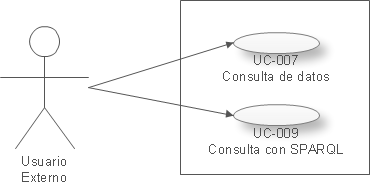
\includegraphics[width=0.6\textwidth]{diagramas_cu/CU_UExterno.png}
    \end{center}
    \caption{Diagrama de CU del Usuario externo}
    \label{fig:DCUAdministrador}
\end{figure}

\subsubsection{Casos de Uso del Administrador}

\begin{figure}[H]
    \begin{center}
        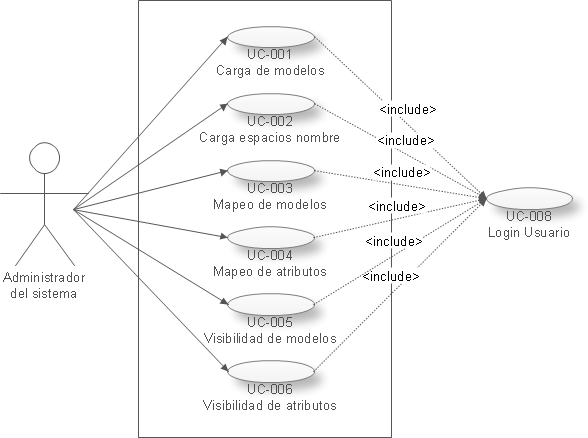
\includegraphics[width=0.8\textwidth]{diagramas_cu/CU_Administrador.png}
    \end{center}
    \caption{Diagrama de CU del Administrador}
    \label{fig:DCUAdministrador}
\end{figure}


\subsection{Descripción de los Casos de Uso}

En este apartado, realizamos una descripción a fondo de cada uno de los Casos de
Uso mostrados anteriormente. Para cada uno de ellos, indicamos los actores que
intervienen en el, la descripción del mismo, posibles flujos alternativos que
puedan darse, y así como la descripción de precondiciones y postcondiciones que
deberán de cumplirse.

\subsubsection{Carga de modelos}

%%%TABLA - Caso de uso 001
\begin{center}
\begin{longtable}{||p{3.4cm}|p{12cm}||}
%primera parte de la tabla
 \hline \hline \bf UC-001 &  \bf Carga de modelos \\
\hline
\endfirsthead
%primera parte de la tabla por pagina
\hline \multicolumn{2}{|r|}{{Continuación de la tabla}} \\ \hline
 \hline \bf UC-001 &  \bf Carga de modelos \\
\hline
\endhead
% ultima parte de la tabla por pagina
\hline \multicolumn{2}{|l|}{{Continúa en la siguiente página}} \\ \hline
\endfoot
% ultima parte de la tabla
\endlastfoot
% DATOS
 \hline \bf Descripción & Carga de modelos y fields del proyecto Django
             donde se va a usar la aplicación.\\
 \hline \bf Referencia & Tabla \ref{tab:caso001}\\
\hline
\hline
\caption{\label{tab:caso001-red} Descripción Caso de Uso - 001 - Carga de modelos} 
\end{longtable}
\end{center}


\subsubsection{Carga de espacios de nombres}

%%%TABLA - Caso de uso 002
\begin{center}
\begin{longtable}{||p{3.4cm}|p{12cm}||}
%primera parte de la tabla
 \hline \hline \bf UC-002 &  \bf Carga de espacios de nombres \\
\hline
\endfirsthead
%primera parte de la tabla por pagina
\hline \multicolumn{2}{|r|}{{Continuación de la tabla}} \\ \hline
 \hline \bf UC-002 &  \bf Carga de espacio de nombres \\
\hline
\endhead
% ultima parte de la tabla por pagina
\hline \multicolumn{2}{|l|}{{Continúa en la siguiente página}} \\ \hline
\endfoot
% ultima parte de la tabla
\endlastfoot
% DATOS
 \hline \bf Descripción & Se debe de realizar una serie de procedimientos los
             cuales permitan a la aplicación cargar la estructura de los
             diferentes namespaces existentes, además de permitir actualizar y
             eliminar estos.\\
 \hline \bf Referencia & Tabla \ref{tab:caso002}\\
\hline
\hline
\caption{\label{tab:caso002-red} Descripción Caso de Uso - 002 - Carga de espacios de nombres}
\end{longtable}
\end{center}


\subsubsection{Mapeo de modelos}

%%%TABLA - Caso de uso 003
\begin{center}
\begin{longtable}{||p{3.4cm}|p{12cm}||}
%primera parte de la tabla
 \hline \hline \bf UC-003 &  \bf Mapeo de modelos \\
\hline
\endfirsthead
%primera parte de la tabla por pagina
\hline \multicolumn{2}{|r|}{{Continuación de la tabla}} \\ \hline
 \hline \bf UC-003 &  \bf Mapeo de modelos \\
\hline
\endhead
% ultima parte de la tabla por pagina
\hline \multicolumn{2}{|l|}{{Continúa en la siguiente página}} \\ \hline
\endfoot
% ultima parte de la tabla
\endlastfoot
% DATOS
 \hline \bf Descripción & Este caso de uso describe el procedimiento mediante
             el cual el administrador del sistema, describe en la aplicación la
             relación de cada uno de los modelos del proyecto Django, con las
             entidades de los distintos namespaces que existen en la
             aplicación.\\
 \hline \bf Referencia & Tabla \ref{tab:caso003}\\
\hline
\hline
\caption{\label{tab:caso003-red} Descripción Caso de Uso - 003 - Mapeo de \mbox{modelos}} 
\end{longtable}
\end{center}


\subsubsection{Mapeo de los atributos}

%%%TABLA - Caso de uso 004
\begin{center}
\begin{longtable}{||p{3.4cm}|p{12cm}||}
%primera parte de la tabla
 \hline \hline \bf UC-004 &  \bf Mapeo de los atributos \\
\hline
\endfirsthead
%primera parte de la tabla por pagina
\hline \multicolumn{2}{|r|}{{Continuación de la tabla}} \\ \hline
 \hline \bf UC-004 &  \bf Mapeo de los atributos \\
\hline
\endhead
% ultima parte de la tabla por pagina
\hline \multicolumn{2}{|l|}{{Continúa en la siguiente página}} \\ \hline
\endfoot
% ultima parte de la tabla
\endlastfoot
% DATOS
 \hline \bf Descripción & Este caso de uso describe el procedimiento mediante
             el cual el administrador del sistema, describe en la aplicación la
             relación de cada uno de los atributos de los modelos del proyecto
             Django, con las propiedades de las entidades de los distintos
             namespaces que existen en la aplicación.\\
 \hline \bf Referencia & Tabla \ref{tab:caso004}\\
\hline
\hline
\caption{\label{tab:caso004-red} Descripción Caso de Uso - 004 - Mapeo de los atributos} 
\end{longtable}
\end{center}


\subsubsection{Establecer visibilidad de modelos}

%%%TABLA - Caso de uso 005
\begin{center}
\begin{longtable}{||p{3.4cm}|p{12cm}||}
%primera parte de la tabla
 \hline \hline \bf UC-005 &  \bf Establecer visibilidad de modelos \\
\hline
\endfirsthead
%primera parte de la tabla por pagina
\hline \multicolumn{2}{|r|}{{Continuación de la tabla}} \\ \hline
 \hline \bf UC-005 &  \bf Establecer visibilidad de modelos \\
\hline
\endhead
% ultima parte de la tabla por pagina
\hline \multicolumn{2}{|l|}{{Continúa en la siguiente página}} \\ \hline
\endfoot
% ultima parte de la tabla
\endlastfoot
% DATOS
 \hline \bf Descripción & Este caso de uso describe el procedimiento que debe
             de seguir el administrador del sistema, para especificar aquellos
             modelos del proyecto Django de los que podrán publicarse los datos.\\
 \hline \bf Referencia & Tabla \ref{tab:caso005}\\
\hline
\hline
\caption{\label{tab:caso005-red} Descripción Caso de Uso - 005 - Establecer visibilidad de modelos} 
\end{longtable}
\end{center}


\subsubsection{Establecer visibilidad de los atributos}

%%%TABLA - Caso de uso 006
\begin{center}
\begin{longtable}{||p{3.4cm}|p{12cm}||}
%primera parte de la tabla
 \hline \hline \bf UC-006 &  \bf Establecer visibilidad de los atributos\\
\hline
\endfirsthead
%primera parte de la tabla por pagina
\hline \multicolumn{2}{|r|}{{Continuación de la tabla}} \\ \hline
 \hline \bf UC-006 &  \bf Establecer visibilidad de los atributos \\
\hline
\endhead
% ultima parte de la tabla por pagina
\hline \multicolumn{2}{|l|}{{Continúa en la siguiente página}} \\ \hline
\endfoot
% ultima parte de la tabla
\endlastfoot
% DATOS
 \hline \bf Descripción & Este caso de uso describe el procedimiento que debe
             de seguir el administrador del sistema, para especificar aquellos
             atributos de los modelos del proyecto Django de los que podrán
             publicarse los datos.\\
 \hline \bf Referencia & Tabla \ref{tab:caso006}\\
\hline
\hline
\caption{\label{tab:caso006-red} Descripción Caso de Uso - 006 - Establecer visibilidad atributos} 
\end{longtable}
\end{center}


\subsubsection{Publicación de los datos}

%%%TABLA - Caso de uso 007
\begin{center}
\begin{longtable}{||p{3.4cm}|p{12cm}||}
%primera parte de la tabla
 \hline \hline \bf UC-007 &  \bf Consulta de datos \\
\hline
\endfirsthead
%primera parte de la tabla por pagina
\hline \multicolumn{2}{|r|}{{Continuación de la tabla}} \\ \hline
 \hline \bf UC-007 &  \bf Consulta de datos \\
\hline
\endhead
% ultima parte de la tabla por pagina
\hline \multicolumn{2}{|l|}{{Continúa en la siguiente página}} \\ \hline
\endfoot
% ultima parte de la tabla
\endlastfoot
% DATOS
 \hline \bf Descripción & Muestra los datos por pantalla usando los estándares
    RDF/XML, RDF/Ntriples, RDF/Turtle, RDFa o Microdata, existentes para la
    publicación de datos en internet.\\
 \hline \bf Referencia & Tabla \ref{tab:caso007}\\
\hline
\hline
\caption{\label{tab:caso007-red} Descripción Caso de Uso - 007 - Consulta de datos} 
\end{longtable}
\end{center}


\subsubsection{Inicio de sesión}

%%%TABLA - Caso de uso 008
\begin{center}
\begin{longtable}{||p{3.4cm}|p{12cm}||}
%primera parte de la tabla
 \hline \hline \bf UC-008 &  \bf Inicio de sesión \\
\hline
\endfirsthead
%primera parte de la tabla por pagina
\hline \multicolumn{2}{|r|}{{Continuación de la tabla}} \\ \hline
 \hline \bf UC-008 &  \bf Inicio de sesión \\
\hline
\endhead
% ultima parte de la tabla por pagina
\hline \multicolumn{2}{|l|}{{Continúa en la siguiente página}} \\ \hline
\endfoot
% ultima parte de la tabla
\endlastfoot
% DATOS
 \hline \bf Descripción & Realiza el login del usuario dentro de la aplicación
        web.\\
 \hline \bf Referencia & Tabla \ref{tab:caso008}\\
\hline
\hline
\caption{\label{tab:caso008-red} Descripción Caso de Uso - 008 - Inicio de sesión} 
\end{longtable}
\end{center}


\subsubsection{Consulta con SPARQL}

%%%TABLA - Caso de uso 009
\begin{center}
\begin{longtable}{||p{3.4cm}|p{12cm}||}
%primera parte de la tabla
 \hline \hline \bf UC-009 &  \bf Consulta con SPARQL \\
\hline
\endfirsthead
%primera parte de la tabla por pagina
\hline \multicolumn{2}{|r|}{{Continuación de la tabla}} \\ \hline
 \hline \bf UC-009 &  \bf Consulta con SPARQL \\
\hline
\endhead
% ultima parte de la tabla por pagina
\hline \multicolumn{2}{|l|}{{Continúa en la siguiente página}} \\ \hline
\endfoot
% ultima parte de la tabla
\endlastfoot
% DATOS
 \hline \bf Descripción & Debe de permitirse al usuario realizar consultas sobre
        los datos utilizando el lenguaje SPARQL.\\
 \hline \bf Referencia & Tabla \ref{tab:caso009}\\
\hline
\hline
\caption{\label{tab:caso009-red} Descripción Caso de Uso - 009 - Consulta con SPARQL} 
\end{longtable}
\end{center}


\subsection{Diagramas de Secuencia}

Una vez hemos descrito cada uno de los casos de uso que deberá incluir la
aplicación, el siguiente paso es plasmar gráficamente el comportamiento de
estos. De esta forma, se muestran a continuación, los diagramas de secuencia de
cada uno de los casos de uso de la aplicación.

\newpage

\subsubsection{UC-001 }

\begin{figure}[H]
    \begin{center}
        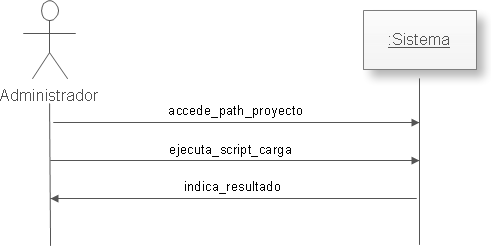
\includegraphics[width=0.75\textwidth]{diagramas_secuencia/DiagramasSecuencia-001.png}
    \end{center}
    \caption{Diagrama de Secuencia CU-001}
    \label{fig:DSCU-001}
\end{figure}

\subsubsection{UC-002 }

\begin{figure}[H]
    \begin{center}
        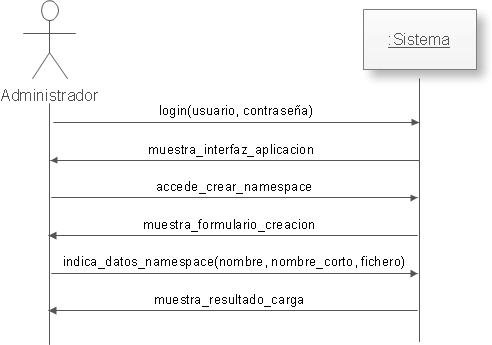
\includegraphics[width=0.7\textwidth]{diagramas_secuencia/DiagramasSecuencia-002.png}
    \end{center}
    \caption{Diagrama de Secuencia CU-002}
    \label{fig:DSCU-002}
\end{figure}

\subsubsection{UC-003 }

\begin{figure}[H]
    \begin{center}
        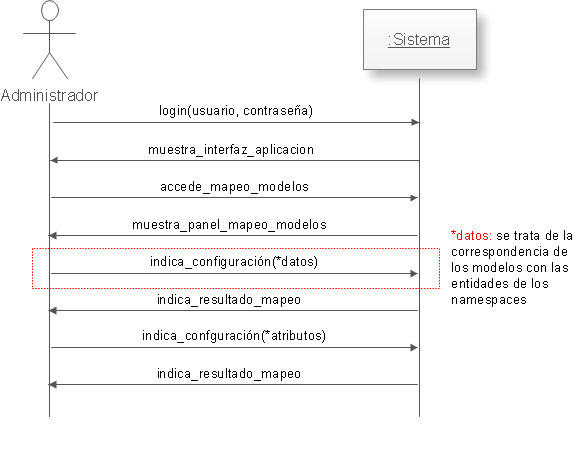
\includegraphics[width=0.7\textwidth]{diagramas_secuencia/DiagramasSecuencia-003.png}
    \end{center}
    \caption{Diagrama de Secuencia CU-003}
    \label{fig:DSCU-003}
\end{figure}

\subsubsection{UC-004 }

\begin{figure}[H]
    \begin{center}
        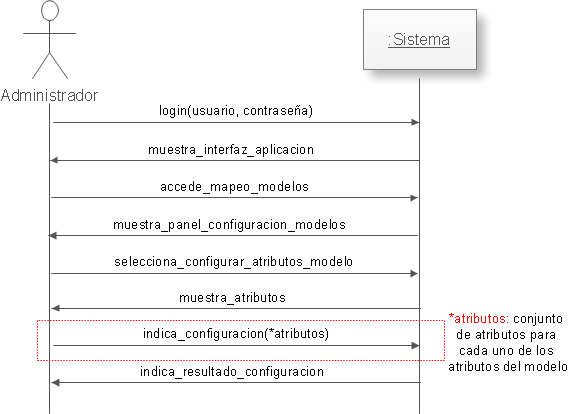
\includegraphics[width=0.7\textwidth]{diagramas_secuencia/DiagramasSecuencia-004.png}
    \end{center}
    \caption{Diagrama de Secuencia CU-004}
    \label{fig:DSCU-004}
\end{figure}

\subsubsection{UC-005 }

\begin{figure}[H]
    \begin{center}
        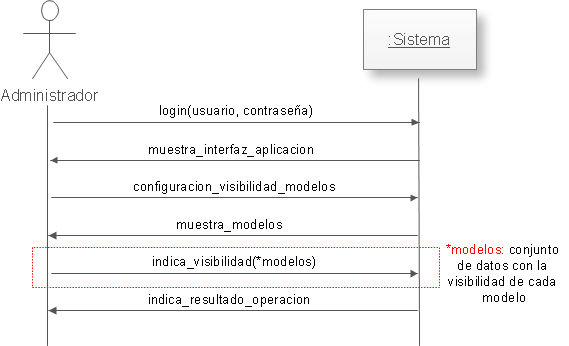
\includegraphics[width=0.75\textwidth]{diagramas_secuencia/DiagramasSecuencia-005.png}
    \end{center}
    \caption{Diagrama de Secuencia CU-005}
    \label{fig:DSCU-005}
\end{figure}

\subsubsection{UC-006 }

\begin{figure}[H]
    \begin{center}
        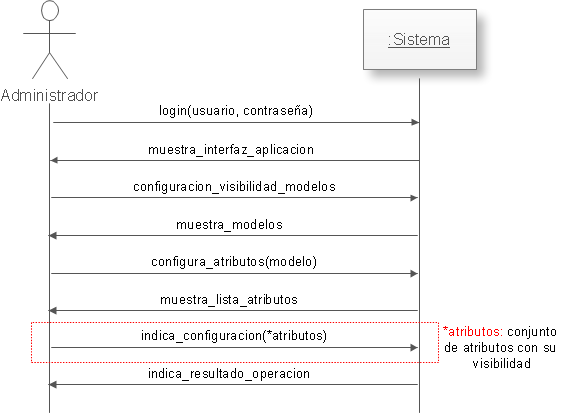
\includegraphics[width=0.8\textwidth]{diagramas_secuencia/DiagramasSecuencia-006.png}
    \end{center}
    \caption{Diagrama de Secuencia CU-006}
    \label{fig:DSCU-006}
\end{figure}
\newpage

\subsubsection{UC-007 }

\begin{figure}[H]
    \begin{center}
        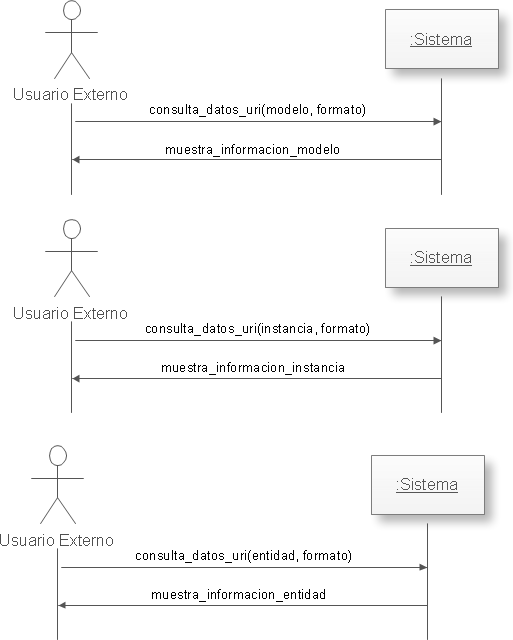
\includegraphics[width=0.8\textwidth]{diagramas_secuencia/DiagramasSecuencia-007.png}
    \end{center}
    \caption{Diagrama de Secuencia CU-007}
    \label{fig:DSCU-007}
\end{figure}

\newpage

\subsubsection{UC-008 }

\begin{figure}[H]
    \begin{center}
        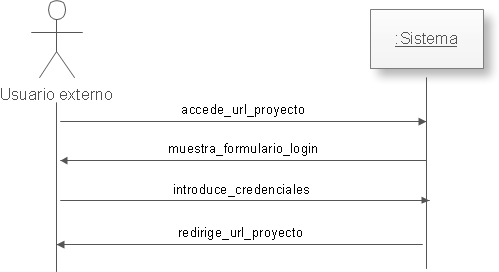
\includegraphics[width=0.8\textwidth]{diagramas_secuencia/DiagramasSecuencia-008.png}
    \end{center}
    \caption{Diagrama de Secuencia CU-008}
    \label{fig:DSCU-008}
\end{figure}

\subsubsection{UC-009 }

\begin{figure}[H]
    \begin{center}
        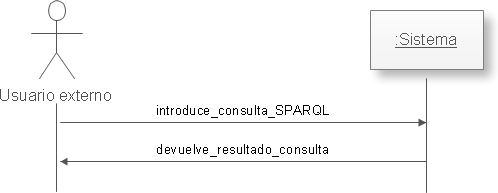
\includegraphics[width=0.8\textwidth]{diagramas_secuencia/DiagramasSecuencia-009.png}
    \end{center}
    \caption{Diagrama de Secuencia CU-009}
    \label{fig:DSCU-009}
\end{figure}


\section{Requisitos de información}

En esta sección se describen los requisitos de gestión de información (datos)
que el sistema debe gestionar. Para ello, utilizando el formato de
especificación propuesto por UML, detallamos a continuación, cada uno de los
requisitos de información de la aplicación:

\subsection{Descripción de los requisitos de información}

%%%TABLA - Requisito Información de los namespaces
\begin{center}
\begin{longtable}{||p{3.4cm}|p{12cm}||}
%primera parte de la tabla
 \hline \hline \bf IRQ-001 &  \bf Información de los namespaces \\
\hline
\endfirsthead
%primera parte de la tabla por pagina
\hline \multicolumn{2}{|r|}{{Continuación de la tabla}} \\ \hline
 \hline \bf IRQ-001 &  \bf Información de los namespaces \\
\hline
\endhead
% ultima parte de la tabla por pagina
\hline \multicolumn{2}{|l|}{{Continúa en la siguiente página}} \\ \hline
\endfoot
% ultima parte de la tabla
\endlastfoot
% DATOS
 \hline \bf Descripción & Se debe almacenar la información acerca de los
             distintos namespaces que almacena la aplicación, de tal forma que
             se tenga la información acerca del namespace, de las entidades que
             componen a este, y de las propiedades que componen a la entidad.\\
 \hline \bf Referencia & Tabla \ref{tab:irq001}\\
\hline
\hline
\caption{\label{tab:irq001-red} Descripción IRQ - 001 - Información de los namespaces} 
\end{longtable}
\end{center}

%%%TABLA - Requisito Información de los modelos
\begin{center}
\begin{longtable}{||p{3.4cm}|p{12cm}||}
%primera parte de la tabla
 \hline \hline \bf IRQ-002 &  \bf Información de los modelos \\
\hline
\endfirsthead
%primera parte de la tabla por pagina
\hline \multicolumn{2}{|r|}{{Continuación de la tabla}} \\ \hline
 \hline \bf IRQ-002 &  \bf Información de los modelos \\
\hline
\endhead
% ultima parte de la tabla por pagina
\hline \multicolumn{2}{|l|}{{Continúa en la siguiente página}} \\ \hline
\endfoot
% ultima parte de la tabla
\endlastfoot
% DATOS
 \hline \bf Descripción & Se debe almacenar la información acerca de los
             distintos modelos que componen al proyecto Django, de tal forma que
             se tenga la información acerca del modelo, y de los fields que
             componen al modelo.\\
 \hline \bf Referencia & Tabla \ref{tab:irq002}\\
\hline
\hline
\caption{\label{tab:irq002-red} Descripción IRQ - 002 - Información de los modelos} 
\end{longtable}
\end{center}


\subsection{Diagrama conceptual de datos}

Una vez que hemos descrito cada uno de los datos que necesitamos que nuestra
aplicación Django almacene, mostramos un diagrama conceptual de datos UML,
donde se puede apreciar como se relacionan cada uno de estos datos entre ellos.
Además, a parte de las distintas clases que almacena la aplicación, podremos
identificar, los atributos, relaciones y restricciones adicionales.

Si observamos el diagrama de clases, está divido en dos partes, numeradas cada
una de ellas. La parte número 1, se corresponde con el requisito de información
\textit{IRQ-001} (Tabla \ref{tab:irq001}), y el apartado número 2, se
corresponde con los requisitos de información descritos en \textit{IRQ-002}
(Tabla \ref{tab:irq002}).

\newpage

\begin{figure}[H]
    \begin{center}
        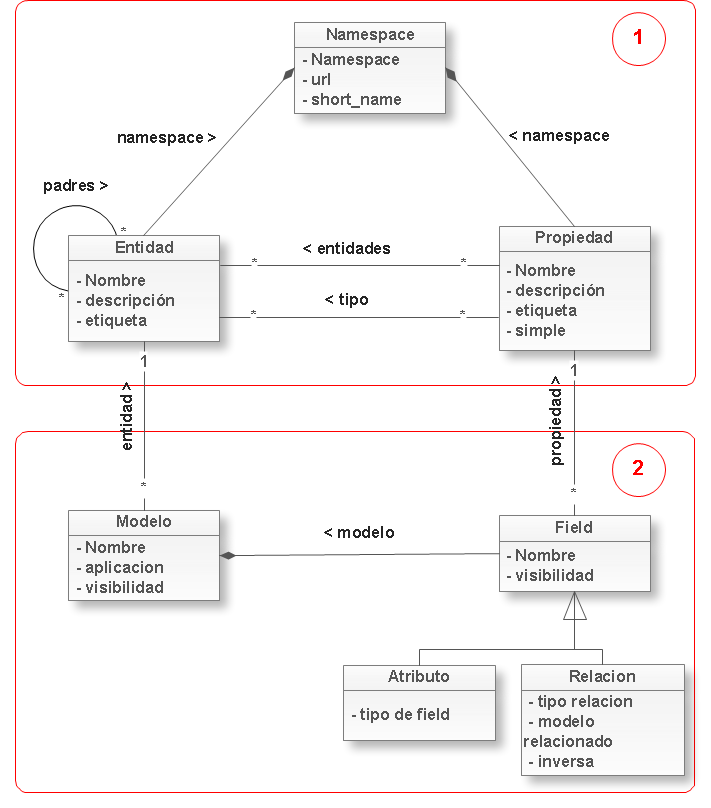
\includegraphics[width=0.9\textwidth]{diagrama_clases.png}
    \end{center}
    \caption{Diagrama conceptual de datos UML}
    \label{fig:ClasesUML}
\end{figure}

\section{Requisitos no funcionales}
\label{sec:RQNF}

A continuación se detalla una descripción de otra serie requisitos, relacionados
con la calidad del software, conocidos como requisitos no funcionales, que el
sistema deberá satisfacer. Estos requisitos son los siguientes:
\begin{itemize}
    \item \textbf{Seguridad:} dicha aplicación no será accesible a usuarios no
           autorizados y solo se publicarán aquellos datos expresamente
           indicados.
    \item \textbf{Estándares de las organizaciones:} deberá de adaptarse a
           cada uno de los estándares impuestos por las distintas organizaciones
           desarrolladoras de las especificaciones para la apertura de datos.
    \item \textbf{Portabilidad:} la aplicación debe de estar diseñada,
           haciendo uso siempre de tecnologías y herramientas independientes de
           la plataforma, de forma que pueda usarse bajo la gran mayoría de
           sistemas operativos actuales.
    \item \textbf{Mantenibilidad:} Esta aplicación se encuentra desarrollada
           como un módulo a parte, de forma que no sea dependiente de un
           proyecto en cuestión. Además, la aplicación deberá de estar
           perfectamente documentada, y se usará la guía de buenas maneras para
           la escritura de código Python PEP8 (\cite{pep8}), de tal forma que
           el código sea lo suficientemente claro.
    \item \textbf{Extensibilidad:} La aplicación debe de ser fácilmente
           extensible, pudiéndose adaptar fácilmente a nuevos estándares para la
           apertura de datos.
    \item \textbf{Interfaz:} La aplicación debe de poseer una interfaz de
           configuración sencilla e intuitiva, de tal forma que un usuario no
           experimentado, pueda aprender a manejarla sin dificultades.
    \item \textbf{Entorno tecnológico:} La aplicación forzosamente debe de
           estar elaborada bajo el lenguaje de programación Python y el
           framework Django, ya que es el principal objetivo de este proyecto,
           proporcionar una herramienta para la apertura de datos en
           aplicaciones Django. El resto de tecnologías a usar, es indiferente,
           siempre y cuando respeten los requisitos que se acaban de imponer.
\end{itemize}


\section{Reglas de negocio}

A lo largo del desarrollo del sistema, además de los distintos requisitos que ha
de cumplir la aplicación, en lo referente a funcionalidades, información o
propiedades que deben de cumplir el sistema, hay que tener en cuenta las
denominadas reglas de negocio, es decir, el conjunto de restricciones, normas o
políticas de la organización que deben ser respetadas por el sistema. A
continuación se detallan, una lista de las distintas reglas de negocio que debe
de cumplir la aplicación:
\begin{enumerate}
    \item El sistema no debe de permitir que un usuario que no posea los
           permisos de administrador, pueda consultar datos, los cuales están
           declarados como privados.
    \item El sistema no permitirá acceder al apartado de configuración de la
           publicación de datos a usuarios que no posean credenciales de
           administrador.
\end{enumerate}

\section{Estudio de alternativas tecnológicas}

La finalidad de este apartado, sería de comentar las diferentes alternativas
tecnológicas que existen, las cuales nos permitirían obtener el producto que
queremos desarrollar, comentando posibles pros y contras de cada una de estas,
de forma que nos ayude a decidirnos por cual de ellas sería la mejor. Aunque en
nuestro caso, no será necesario definir estas, ya que el principal objetivo de
este proyecto informático, es el de dotar de una cierta cualidad (apertura de
datos en internet) a una tecnología en concreto (Django), por lo que no tendría
sentido en un principio estudiar otras alternativas tecnológicas.

\section{Análisis GAP}

Este proyecto no se encuentra basado en ningún software base, ya que vamos a
realizar una aplicación software completamente desde cero. Si cabe comentar, que
el proyecto se va a realizar en Python, para el framework Django, por lo que si
considerásemos el framework Django como un software base a partir del cual vamos
a desarrollar nuestro proyecto, este nos proporciona una serie de herramientas
las cuales nos simplificarán el desarrollo del mismo. Entre todas estas
herramientas que comentamos, cabría destacar las siguientes:
\begin{itemize}
    \item Herramientas para el acceso a los distintos modelos de las
           aplicaciones. Esto nos facilitará enormemente la introspección que
           deberemos de realizar, para captar los modelos de los que se
           encuentran compuestos los proyectos Django.
    \item Herramientas para la gestión de las sesiones y del log de la
           aplicación.
    \item Herramientas para la generación de formularios, incluyendo
           comprobaciones de seguridad ante distintos tipos de ataques.
    \item Manejador propio para las bases de datos, con un lenguaje propio de
           consultas, de tal forma que podemos realizar la aplicación de forma
           que esta sea completamente independiente del SGBD que use el proyecto
           donde vaya a ser implantada la aplicación.
    \item Una comunidad, la cual proporciona un soporte continuo del framework
           Django.
\end{itemize}

El proyecto aunque no toma como base para su desarrollo la plataforma D2Rq,
genera ficheros de configuración para ésta, por lo que para el desarrollo de
este módulo se ha debido de realizar un estudio del funcionamiento de esta
plataforma, y adaptar la generación del fichero de configuración a ésta. La
plataforma D2Rq, es de código abierto, y proporciona un sistema para el acceso a
los datos de bases de datos relacionales, como si se tratasen de grafos RDF
virtuales de solo lectura. De esta forma, ofrece a los usuario acceso mediante
RDF al contenido relacional de las bases de datos, sin la necesidad de tener que
replicar estos sobre un almacenamiento en formato RDF.
